%trascrizione: Costa
%metto sempre il simbolo di vettore?
% risposta: no, in effetti mi sa che ho fatto una cazzata nella lezione precedente, il simbolo di vettore sarebbe da usare quando si fa riferimento alla struttura vettoriale in particolare, mo' li tolgo.
%devi parlare del modello a semipiano
% risposta: se era nella mia lezione, mi sa che me lo sono perso, se tu ce l'hai mettilo.

\titlet{Funzioni a foruncolo}

\begin{defn}[Funzione a foruncolo]
	Dati $b>a>0$, una funzione liscia
	$\fundef[\lambda] {\R^n}{\R}$
	che dipende solo da $|x|$ tale che 
	\begin{itemize}
		\item $|x|\le a\implies\lambda(x)=1$;
		\item $a<|x|<b\implies0<\lambda(x)<1$;
		\item $|x|\ge b\implies\lambda(x)=0$
	\end{itemize}
	è detta \emph{funzione a foruncolo} (o anche \emph{partizione dell'unità di Paley-Littlewood}).\footnotemark
	\footnotetext{In fondo alla dimostrazione del lemma di Morse (\autoref{th:lemmamorse}) c'è un esempio di come costruire funzioni di questo tipo.}
	\begin{figure}
		\centering
		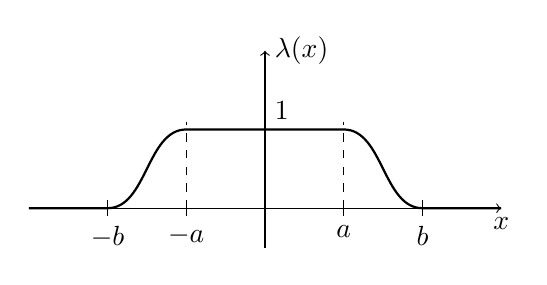
\begin{tikzpicture}
			\pgfmathsetmacro\a{1}
			\pgfmathsetmacro\b{2}
			\pgfmathsetmacro\h{(\a+\b)/2}
			\draw[->] (0,-.5) -- (0,2) node[right] {$\lambda(x)$};
			\draw[->] (-3,0) -- (3,0) node[below] {$x$};
			\foreach \x in {,-} {
				\draw (\x\a,-.1) node[below] {$\x a$} -- (\x\a,.1);
				\draw (\x\b,-.1) node[below] {$\x b$} -- (\x\b,.1);
				\draw[dashed] (\x\a,0) -- (\x\a,1.1);
				\draw[thick] (\x3,0) -- (\x\b,0) .. controls (\x\h,0) and (\x\h,1) .. (\x\a,1) -- (0,1);
			}
			\path (0,1) node[above right] {$1$};
		\end{tikzpicture}
		\caption{Funzione a foruncolo $\R\funarrow\R.$}
	\end{figure}
\end{defn}

\begin{oss}
 Nei punti in cui $\abs x = a$ tutte le derivate sono nulle, dunque $\lambda$ non è analitica.
\end{oss}

% questa cosa mi sembra senza senso, la sostituisco con supercazzola generica
% Usiamo adesso questa nozione per estendere funzioni definite localmente.
% \begin{prop}
%  Sia $M$ una varietà e $(U, \phi)$ una carta. Allora posso estenderla su tutta la varietà.
% \end{prop}
%  \begin{proof}
%   Basta considerare $\fundef[\lambda\cdot f] M\R$ con $\lambda$ a foruncolo.
%  \end{proof}

Le funzioni a foruncolo si usano per estendere funzioni lisce $U\subseteq\R^n\funarrow\R^k$ a tutto $\R^n$:
se il dominio contiene una palla, si moltiplica la funzione per una funzione a foruncolo che sia nulla fuori dalla palla.
 
\titlet{Varietà con bordo}
Per definire le varietà come oggetti che localmente somigliano a $\R^n$, abbiamo usato omeomorfismi locali con aperti di $\R^n$.
Per definire le varietà con bordo, considereremo omeomorfismi locali con aperti di un sottoinsieme di $\R^n$ che abbia bordo.
In particolare useremo il \emph{semipiano superiore}:
\[\mathbb H^n\is[0;\infty)^n=\setdef[x\in\R^n]{\forall i:x_i\ge 0}\]

\begin{defn}[Diffeomorfismo fra sottoinsiemi arbitrari di $\R^n$]
	\label{th:arbdiffeo}
Sia $\fundef AB$ con $A,B\subseteq \R^n$. $f$ è un \emph{diffeomorfismo} se
\begin{itemize}
 \item è un omeomorfismo;
 \item $\forall x\in A \,\exists (U_x,\phi)$ carta locale di $\R^n$ tale che $f|_{U\cap A}=\phi|_{U\cap A}$.
\end{itemize}
\end{defn}

\begin{defn}[Varietà con bordo]
 $M$ è una \emph{$n$-varietà con bordo} se 
 \begin{itemize}
  \item è uno spazio topologico $T_2$ e 2-numerabile;
  \item è munito di atlante massimale $\set{(U_\lambda,\phi_\lambda)}$ a valori in $\mathbb H^n$, cioè si ha $\fundef[\phi_\lambda]{U_\lambda}{W_\lambda}$ omeomorfismo con $U_\lambda$ aperto di $M$ e $W_\lambda$ aperto di $\mathbb H^n$;
  \item $\forall \mu,\lambda: \phi_{\mu}\circ\phi_{\lambda}^{-1}:\phi_{\lambda}(U_{\lambda}\cap U_{\mu})\funarrow\phi_{\mu}(U_{\lambda}\cap U_{\mu})$ è un diffeomorfismo nel senso della \autoref{th:arbdiffeo}.
 \end{itemize}
\end{defn}
\begin{defn}[Bordo]
	Il \emph{bordo} di una $n$-varietà con bordo $M$ è costituito dai punti la cui immagine attraverso una carta è contenuta nella frontiera del semipiano superiore:
	\begin{gather*}
\boundary M \is \setdef[x\in M]{\exists(U_x,\phi)\text{ carta locale}:\phi(x) \in \bound \mathbb H^n} \\
\bound \mathbb H^n = \mathbb H^n \cap \setdef[x\in\R^n]{\exists i:x_i=0}
\end{gather*}
	Può essere $\boundary M=\nullset$, nel qual caso diciamo che $M$ è senza bordo o \emph{chiusa}.
\end{defn}
\begin{ex}
 Se un punto è di bordo per una carta, lo è per tutte le carte che lo contengono.
\end{ex}
\begin{fat}
	Le nozioni di applicazione liscia e quindi di diffeomorfismo si estendono alle varietà con bordo.
\end{fat}

\subtitlet{Sottovarietà}

\begin{defn}[Sottovarietà]
 Una \emph{sottovarietà} $N^n$ di $M^m$ varietà con $\partial M = \nullset, N\subseteq M (n\le m)$ se $\forall x\in N, \exists$ carta locale di $x \in M$ con $\fundef[\phi] U\R^m $
\end{defn}
\begin{defn}[Punto regolare]
 $y$ è un \emph{punto regolare} per $f$ se $\forall x\in f^{-1}(y)$, $\de_xf$ è surgettiva.
\end{defn}
\begin{prop}
 $y$ punto regolare $\implies f^{-1}\is N$ è sottovarietà di $U$.
\end{prop}
\begin{proof}
 Segue da funzione implicita in forma surgettiva.
 \begin{figure}
  \centering
  \input{diffeo.pdf_tex}
  \caption{la nuova carta "vede dritto!"}
 \end{figure}

\end{proof}
\begin{prop}
 $\fundef[f] U\R^m$, $U$ aperto di $\R^n$. Se $\forall x \in U, \de_xf$ iniettiva, $f$ omeomorfismo$\implies N\is f^{-1}(y)$ è sottovarietà di $\R^n$ e f diffeomorfismo.
\end{prop}
\begin{proof}
 Segue da funzione implicita in forma iniettiva
\end{proof}
\begin{oss}
 Nel teorema sopra l'ipotesi di omeomorfismo è necessaria!
 Come controesempio basta prendere:
 \begin{center}
  \centering
  \input{trifoglio.pdf_tex}
 \end{center}
 Nel cerchio tratteggiato si ha il problema: ci sono 3 "rami"!
 \marginpar{non rieso a mettere bene la figura :(}
\end{oss}
Si osservi che abbiamo tre modelli possibili al variare del domicilio di una  $n$-sottovarietà contenuta in una $m$-varietà ($n\le m$):
\begin{itemize}
 \item Il bordo sta nel bordo (1).
 \item Il bordo di $\mathbb H^n$ non sta nel bordo di $\mathbb H^m$ (2).
 \item Caso misto (3).
\end{itemize}
\begin{center}
 \input{modellobordo.pdf_tex}
\end{center}

\begin{defn}[Sottovarietà propria]
 $N\in M$ è \emph{sottovarietà propria} se l'unico modello che si realizza è (1), ossia $\partial N = N\cap \partial M$.

\end{defn}
